\documentclass{article}
\usepackage{graphicx}
\graphicspath{{./images/}}
\usepackage{geometry}
\usepackage{hyperref}
\usepackage{paralist}
\usepackage[round]{natbib}
\usepackage{sectsty}
\usepackage{gensymb}
\usepackage{caption}
\usepackage{subcaption}
\usepackage{listings}
\usepackage[space]{grffile}
\usepackage{latexsym}
\usepackage{amsfonts,amsmath,amssymb}
\usepackage{url}
%\usepackage{minitoc}
\hypersetup{colorlinks=false,pdfborder={0 0 0}}
\usepackage{textcomp}
\usepackage{longtable}
\usepackage{multirow,booktabs}
\newcommand{\truncateit}[1]{\truncate{0.8\textwidth}{#1}}
\newcommand{\scititle}[1]{\title[\truncateit{#1}]{#1}} 
\usepackage[parfill]{parskip}

% Typeface
\usepackage{ifxetex}
\ifxetex
  \usepackage{fontspec}
  \defaultfontfeatures{Ligatures=TeX} % To support LaTeX quoting style
  \setmainfont[Mapping=tex-text, Color=textcolor]{HelveticaNeue}
  %\setmainfont[Mapping=tex-text, Color=textcolor]{Avenir LT Std}
\else
  \usepackage[T1]{fontenc}
  \usepackage[utf8]{inputenc}
  \renewcommand{\familydefault}{\sfdefault}
  \usepackage{helvet}
\fi
%\chapterfont{\Large} % \sffamily
%\renewcommand{\chaptername}{}
%\renewcommand{\thechapter}{}

% Title page
\usepackage{xcolor}
\definecolor{titlepagecolor}{cmyk}{0,0,0,0}
\definecolor{namecolor}{cmyk}{0,0,0,1} 
\definecolor{chaptertitlepagecolor}{cmyk}{0,0,0,0.9}
\definecolor{chapternamecolor}{cmyk}{0,0,0,0.3}  

% GRASS GIS version for URLs and commands
\newcommand{\grassversion}{70}
% GRASS GIS project base URL
\newcommand{\grassbaseurl}{http://grass.osgeo.org}
% GRASS GIS module
\newcommand{\gmodule}[1]{\href{\grassbaseurl/grass\grassversion/manuals/#1.html}{\emph{#1}}\index{#1}}
% GRASS GIS addon module
\newcommand{\gaddon}[1]{\href{\grassbaseurl/grass\grassversion/manuals/addons/#1.html}{\emph{#1}}\index{#1}}
\newcommand{\filename}[1]{\texttt{#1}}

\begin{document}

%---------------------------------------------- TITLE PAGE ----------------------------------------------
%\begin{titlepage}
%\newgeometry{left=7.5cm} %defines the geometry for the titlepage
%\pagecolor{titlepagecolor}
%\noindent
%%\includegraphics[width=2cm]{images/sage.pdf}\\[-1em]
%%\includegraphics[width=2cm]{images/sage.png}\\[-1em]
%\color{black}
%\textbf{\textsf{Brendan Alexander Harmon}}\\
%\makebox[0pt][l]{\rule{1.3\textwidth}{1pt}}
%\par
%\noindent
%%\textbf{\textsf{North Carolina State University}} \textcolor{namecolor}{\textsf{PhD in Design}}
%%\textbf{\textsf{Brendan Alexander Harmon}} 
%\textcolor{namecolor}{\textsf{North Carolina State University}}
%\vfill
%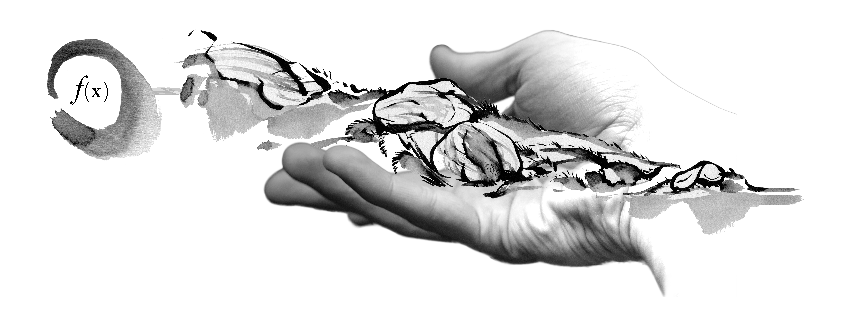
\includegraphics{images/tangible_landscape_diagram.pdf}
%%\includegraphics[width=\textwidth]{images/procedural_landscape.png}
%\vfill
%\noindent
%{\huge \textsf{Tangible Landscape}}
%\vskip\baselineskip
%\noindent
%\textsf{October 2015}
%\end{titlepage}
%\restoregeometry % restores the geometry
%\pagecolor{white}

%---------------------------------------------- LIT REVIEW TITLE ----------------------------------------------

\begin{titlepage}
\newgeometry{left=7.5cm} 
\pagecolor{chaptertitlepagecolor}
\noindent
\color{white}
%\textbf{}
\large
%\textcolor{chapternamecolor}
{\textsf{Embodied cognition in tangible computing}}\\ 
\makebox[0pt][l]{\rule{1.3\textwidth}{1pt}}
\par
\noindent
\textcolor{chapternamecolor}
{\textsf{Literature review}}\vfill
%\noindent
%{\huge \textsf{Literature review}}
%\vskip\baselineskip
%\noindent
%\textcolor{chapternamecolor}{\textsf{Tangible Landscape}}
\end{titlepage}
\restoregeometry % restores the geometry
\pagecolor{white}

%---------------------------------------------- TOC ----------------------------------------------

\tableofcontents
\pagebreak

%%%%%%%%%%%%%%%%%%%%%%%%%%%%%%%%%%%%%%%%%%%%%%%%%%%%%%%%

\section{Introduction}

% cognitive science
Emerging theories of cognitive science rethink how we interact with our environment, tools, and computers 
and have inspired new modes of computing. 
% design theory
Based on the theories of embodied, situated, and distributed cognition 
researchers have theorized a physical-digital divide in human-computer interaction --
positing that 
the high level of abstraction required to interact with a computer in a visual computing paradigm 
constrains how we think -- 
% implementation
and designed innovative technologies for bridging this divide such as tangible user interfaces (TUIs). 
TUIs are designed to enable embodied cognition % situated and distributed
by physically manifesting data so that we can kinaesthetically sense and tangibly interact with computations.
% implications for spatial thinking and education
More embodied cognition in computing should enhance spatial thinking and may also encourage creative thinking.

% purpose
While these theories have inspired the design of novel technologies for human-computer interaction,
their applied principles need to be empirically tested, critiqued, and refined in order to improve interaction design.  
This research studies how tangible computing mediates spatial and creative thinking in order to improve interaction design and enhance spatial performance. 
% overview
This literature review begins with a critical overview of 
emerging theories of cognitive science and the theories of human-computer interaction that they have inspired.
Then the implementation of these theories of human-computer interaction is explored 
in a critical review of the evolution of TUIs. 
% agenda
After a review of research on tangible interaction a research agenda is proposed.

%The theory of embodied cognition, cognition functionally embedded in and distributed through the body, has inspired tangible computing, a new paradigm of human-computer interaction. 
%Situated cognition, cognition functionally embedded in a sociocultural context, has framed computing as a social process.
%Distributed cognition, cognition distributed across networks of agents and artifacts, reframes the role of technology in cognition as a functional part of the way we think. 

%\clearpage

%%%%%%%%%%%%%%%%%%%%%%%%%%%%%%%%%%%%%%%%%%%%%%%%%%%%%%%%

\section{The cognitive science of human-computer interaction}

\subsection{Embodied, situated, and distributed cognition}
There is a new paradigm of cognitive science that studies `cognition beyond the brain' \citep{Hardy-Vallee2008}. 
This new paradigm -- embodied, situated, and distributed cognition -- explores how 
cognition is functionally embedded in the body, embedded in its environment, and distributed across networks of agents and artifacts. 
While older paradigms of cognitive science studied the mind abstracted in isolation, this paradigm grounds cognition in its biocultural context studying how a continuous flow of information links brain, body, and environment \citep{Hardy-Vallee2008}.

% embodied cognition
In embodied cognition the mind is embedded in the body. It is based on bodily experience. 
Higher cognitive processes, the traditional realm of cognitive science, rely on lower level processes
such as emotion and sensorimotor processes that link perception and action \citep{Hardy-Vallee2008}. 
Thus our bodies and actions mediate how we think. We can for example physically simulate cognitive processes, offloading cognition onto action to functionally `think with our bodies' \citep{Kirsh2013}. 
We can cognitively grasp objects, temporarily, contingently incorporating tools into our body schema \citep{Kirsh2013}.
This view of cognition considers feeling, action, and perception to be functionally integral to thought.

% situated cognition
In situated cognition the mind is embedded in its environment. 
Situated cognition is a sociocultural process influenced by environment, society, and culture. Information not only flows into the body and thus the mind from its environment, but also from the mind via the body into the environment.
Since information can be stored in and transformed by the environment
we use our environment, our artifacts, and our tools to store ideas, to offload cognitive processes, but our environment, our artifacts, and our tools also constrain and transform our ideas, mediating cognition. 
By storing ideas or mental states in external representations like writing or painting
we can extend our memory, but -- given the constrains of the medium -- we can also transform the idea or state through its expression. 
In addition to reducing our cognitive load by offloading cognitive processes onto our bodies or our environments \citep{Wilson2002} 
we can also enhance our cognitive performance by offloading onto technology -- technology such as language, books, telecommunications, and computing \citep{Dror2008}. 
Thus cognition is grounded in, uses, transforms, and is transformed by its environment \citep{Hardy-Vallee2008,Anderson2008}.
Since from a phenomenological perspective meaning arises from interaction with the environment \citep{Dourish2001}
situated cognition studies how interaction and thus meaning is mediated by the environment, artifacts, and tools \citep{Reichelt2008}. 

% distributed cognition
In distributed cognition the mind is distributed across sociocultural and technological networks. It is distributed across networks of situated agents and artifacts through language, technology, society and culture \citep{Hardy-Vallee2008}. 
The means of communication, of shared thought, mediate meaning and cognition.  

%Embodied cognition is the theory that some cognitive processes are rooted in action and perception \citep{Wilson2002}. 
%In this paradigm cognition is theorized to be situated in its context, be constrained by time, be distributed, use its environment, be motivated by action, and use the body to think. %\citep{Wilson2002} 
%% situated cognition
%Embodied cognition is situated in its context, in the body and its environment, in time and space. 
%Meaning arises from interaction with the environment 
%and thus cognition is rooted in action and perception, the means of interaction \citep{Dourish2001}. 
%% distributed
%Furthermore embodied cognition is distributed between oneself and the environment, across time, and through social networks. 

% situated cognition critiqued
Some of these ideas are controversial. 
When we perform a task our cognition is situated in the immediate context, 
but when we think abstractly without a task to perform we are do not have an immediate context \citep{Wilson2002}. From this perspective abstract thinking is not situated. 
From a phenomenological perspective, however, all meaning is derived from interaction
making even abstract thinking grounded -- situated -- in phenomenological experience \citep{Dourish2001}.  
Even from this more philosophic perspective abstract thinking should be less situated than the thinking that directs an action, the cognition for performing a task. However, even when thinking abstractly we often rely on our bodies and sometimes our environment. We may physically simulate what we imagine, representing for example a shape with our hands, measuring a distance with our bodies, or counting off a sequence with our fingers \citep{Wilson2002}. 
% spatial cognition
Spatial thinking -- whether abstract or applied -- is situated. We think about space visually and kinaesthetically. We visualize and feel it. 

% distributed cognition critiqued
%Distributed cognition has been criticized for conceptualizing cognition too broadly. \citeauthor{Dror2008} argues that we should define cognition narrowly as a mental state in order to avoid vagueness.
%Given this narrow definition of cognition when we can offload thinking to cognitive technologies, the technologies -- lacking mental states -- do not think and are thus not part of a distributed cognitive process \citep{Dror2008}. 

% online and offline cognition
\citeauthor{Wilson2002} draws a distinction between online embodied cognition for immediate tasks requiring action and offline embodied cognition for tasks that are either imaginary or distant in time or space \citeyearpar{Wilson2002}. 
Many tasks are time sensitive and require fast thinking. 
The need to act quickly can cause representational bottlenecks -- mental models may not be formed quickly enough for one to succeed at a task. 
Online embodied cognition uses the body and environment to think quickly. 
We can reduce our cognitive load and mental modeling time with our bodies by learning motor schema or pragmatic representations that let us automatically, subconsciously perform tasks. 
We can also cognitively offload by using our bodies or our environment as a proxy for memory. 
When an action or our environment is indexical to the task we cognitively offload online. 
When, however, the relationship between our environment and the task is symbolic we cognitively offload offline. 
When for example we draw, write, or diagram the relationship between the physical representation and the idea is symbolic and disconnected in time and sometime space. 
Symbolic cognitive offloading is offline and yet embodied, grounded in tools or our environment. 
Thus offline cognition, while often abstract, can also be embodied. 
Mental simulations can also be embodied as they may draw upon visual, auditory, and kinesthetic representations derived from experience \citep{Wilson2002}. 

% archiving
We can also archivally offload onto our environment by encoding ideas for example in books, maps, and places \citep{Wilson2002}.
Basso for example describes from an anthropological perspective how meaning and cultural significance can be invested in a landscape and how the cultural values embedded in that landscape can inspire introspection and learning across generations \citeyearpar{Basso1996}. 
% implications for computing
A computer, however, is not just a tool for storage, for archiving data -- it is a tool for computation, for enhancing our thinking, for augmenting our cognitive processes \citep{Dror2008}. 
We use it to extend our thinking capacity, to process, model, simulate, and represent complex phenomena. 

% Enactive perception: `we cocreate our perceived environment, so perception itself is a form of action.'

% Enactive landscape: `the structure an agent cocreates with the world when he or she acts in a goal-oriented manner.'

% Enactive landscape: `the set of possibilities that can in principle be brought into being when an agent interacts with an underlying environment while engaged in a task or pursuing a goal.'

\subsection{Embodied interaction}
The theses
that cognition is embodied and situated,
that we sometimes understand more through acting than by watching,
that tools mediate how we perceive, think, and act, 
and that tools like computers can extend our capacity to think \citep{Kirsh2013}
have inspired a new paradigm of human-computer interaction -- embodied interaction.  

% history
\citeauthor{Dourish2001} 
outlined the history of human-computer interaction as an evolution from electrical to symbolic to textual to visual computing 
and theorized that the emerging paradigms of tangible and social computing would 
make interaction more embodied and situated \citeyearpar{Dourish2001}.

% premise
The dominant paradigm of computing today -- visual computing, computing via a graphical user interface (GUI) -- 
is thought to be relatively disembodied because of the high level of abstraction required to interact with the computer. 
The body plays a limited role in visual computing. 
% graphical user interfaces 
With a GUI one uses an input device to interact with data visually represented as graphics on a display. 
When we use a mouse and keyboard, archetypal examples of input devices, there is a disjunction between our actions and the results -- the double click of a mouse button is not indexical to its result, the opening of a folder. This arbitrary coding adds a layer of abstraction between our intention and its expression. 
Input devices include mice and keyboards, touch sensitive displays, and digitizing pens. Some of these, the pressure-sensitive digitizing pens for example, enable a wider range of haptic experience and enaction. The more haptic feedback a GUI offers, the closer to a TUI it becomes.
Inputs are limited to keystrokes or two-dimensional translations of pointing devices like mice or digitizing pens.
Feedback -- save for the position of the hand on the pointing device in relation to a cursor in an abstract space -- is visual 
\citep{Dourish2001,Ishii2008}. 
Even the transitional paradigm of touch computing is limited to two-dimensional touch gestures and visual or symbolic feedback. 
There is a disconnect between intention, action, and feedback -- 
our intention is translated into symbolic action, action into computation, computation into visual representation, and representation into mental model. 
Multiple layers of abstraction separate intention, enaction, and a critical understanding of the result. 
% implications of disembodiment
The limited forms of input and feedback in visual computing 
enable sophisticated, abstract thinking, but do not afford many aspects of embodied cognition like cognitive grasping, haptic shape recognition, and physical simulation. 

% unsituated
Furthermore visual computing is thought to be relatively unsituated as it immerses users in abstract, disembodied virtual environments disconnected from their immediate, physical environments. Social interaction in virtual environments lacks the cues and affordances of natural social interaction in physical environments. 
Ubiquitous computing was a vision of computation embedded in our everyday, physical environment, of situating computing in our physical and social environment rather than immersing ourselves in abstract digital environments \citep{Dourish2001}. This vision of computationally enhanced everyday life inspired tangible computing \citep{Ishii1997}. 

% problem
The relatively disembodied nature of visual computing has been described as a physical-digital divide, 
a disconnect between `cyberspace and the physical environment' \citep{Ishii1997}. 
% experimental design agenda
Human-computer interaction researchers and designers have sought 
to bridge the physical-digital divide with tangible computing.
Tangible computing aims to embody computing 
by coupling physical and digital data \citep{Dourish2001} -- 
by physically manifesting digital data so that we can cognitively grasp and absorb it,
so that we can think with it rather than about it \citep{Kirsh2013}. 
\citeauthor{Ishii1997} envisioned that TUIs would  `take advantage of natural physical affordances to achieve a heightened legibility and seamlessness of interaction between people and information' \citeyearpar{Ishii1997}. 

% Tangible user interfaces
Many TUIs have been designed and prototyped including 
the Marble Answering Machine \citep{Poynor1995},
Urp \citep{Underkoffler1999},
the Aegis Hyposurface \citep{Goulthorpe2000}, 
FEELEX \citep{Iwata2001}, 
Luminous Table \citep{Ishii2002}, 
Illuminating Clay \citep{Piper2002a}, 
Sandscape \citep{Ishii2004}, 
the Tangible Geospatial Modeling System \citep{Tateosian2010},
Relief \citep{Leithinger2010}, 
inFORM \citep{Follmer2013}, 
and
the Augmented Reality Sandbox \citep{Kreylos2015}.
% research
Research on TUIs, however, has largely been limited to 
user feedback (such as \citealt{Ishii2004}),
case studies (such as \citealt{Iwata2001,Ishii2002,Tateosian2010}),
and small scale qualitative studies using methods like protocol analysis (such as \citealt{Kim2008}).

% research agenda 
A better understanding of the cognitive implications of embodiment and disembodiment in computing would improve interaction design. 
To understand how computing transforms cognition we need to study
`the complex coordination between external and internal simulation, between doing things internally and doing things externally' \citep{Kirsh2013}. 
The theory of embodied interaction needs to be rigorously tested, critiqued and refined so that 
we can develop more nuanced design principles that are derived from theory grounded in empirical research. 
The assumption that the more human-computer interaction is embodied, 
the more natural it will be needs to be refined and nuanced.  
Intermediate levels of `realism' in embodied interaction, for example, may lead to a disconcerting `uncanny valley' of expectation disappointed giving rise to uncertainty and misinterpretation. If some aspects of an interaction closely mirror physical reality, while others are still highly abstract, users may experience a cognitive dissonance for the appearance of reality in one aspect suggests it in another. Therefore the coherence and consistency of experience may be more important than the relative embodiment of any aspect
\citep{Cafaro2014}. 

Theoretically tangible computing is especially well suited to spatial applications, but it has also been used for aspatial applications such as tangible programming \citep{Horn2007}.
Given that visual computing already enables sophisticated abstract thinking, 
embodied interaction through tangible computing 
may not add any cognitive potential in some computing applications. 
A study of the coordination of internal and external simulation and processing 
may show which applications embodied interaction enhances and how. 
Furthermore we should study the degree to which abstract and embodied thinking can be coordinated by coupling visual and tangible computing. 

\subsection{Object-oriented action}
% action and cognition

% object-oriented action and tool use
In cognitive neuroscience actions such as reaching for, grasping, manipulating, and using an object are considered object-oriented. 
To interact with an object, to use a tool -- to sculpt sand or move a mouse -- we need to understand where the object is relative to us in space, understand its form and physical properties, and identify what we do can with it. 
Using a tool is a question of space, mechanics, and semiotics. 

% pragmatic and semantic representations
We use internal models to generate action -- to predict and react to known stimuli and adapt to and learn from novel stimuli. 
Object-oriented action is directed by both pragmatic and semantic representations, subconscious and conscious internal models based on haptic and visual feedback \citep{Jeannerod1997}. 

% pragmatic representation
Pragmatic representations are internal models for rapidly generating action
that are primarily based on haptic or tactile feedback. 
% haptic feedback
We use touch to directly assess the form and physical properties of objects -- their size, shape, volume, weight, hardness, and texture. 
This haptic feedback is processed automatically, immediately, and subconsciously \citep{Jeannerod1997}. 

% semantic representation
Semantic representations assign meaning and cognitively signal action. 
They are primarily based on visual perception \citep{Jeannerod1997}.
% visual feedback
Vision, however, requires interpretation and is subject to illusions.
Visually perceived depth is reconstructed from perspective, accommodation and vergence, interposition and shading, and motion parallax.
In stereoscopic vision we derive the visual third dimension from perspective based on the difference between the two-dimensional imagery projected to each eye. 
Aspects of perspective include size, linear position, perceived distance, and textural perspective. 
Illusions can arise from misreading curvature, misjudging distance, and misapproximating size based on distance \citep{Howard2012b,Howard2012c, Jeannerod1997}. 
Since visual feedback is cognitively processed for interpretation the derived semantic representation is subjective and mediated by knowledge. 
Visually perceived objects are semantically classified and identified based on their perceived, phenomenological attributes \citep{Jeannerod1997}. 

% parallel processing
Action can be driven by both pragmatic and semantic representations that are coordinated as they unfold on different timescales. 
Both types of representation are processed in parallel, exchange information, and are temporally coordinated. 
When for example we try to identify an object by both feeling it and seeing it we are simultaneously processing haptic and visual feedback. The pragmatic and semantic representations inform each other, but there is a temporal disjunction due to the latency in processing visual feedback so they are coordinated by a higher level temporal schema \citep{Jeannerod1997}. 

% semiotics
To use a tool we need to be able to identify it and what it can do. 
A tool may afford many different actions; we may be able to use it in many different ways, but we may not realize all of them. 
The affordances of a tool -- the actions we think we can do with it \citep{gibson1977} -- are mediated by our knowledge and experience.
Therefore knowing how to use an object can be a cognitive task based on a semiotic understanding of what it is and what it can do. 
It can also be a exploratory procedure based on pragmatic action \citep{Jeannerod1997}. Action can be informed by a continuum from innate properties to symbolic meanings. 

% implications for hci
The neuroscience of object-oriented action supports in theory the idea that TUIs can offer affordances that GUIs cannot.
This design idea, proposed by \citet{Ishii1997}, has driven the development of tangible computing.
\citeauthor{Ishii1997} criticized visual computing -- arguing that ``GUIs fall short of embracing the richness of human senses and skills people have developed through a lifetime of interaction with the physical world'' -- and proposed a vision of TUIs ``to bridge the gaps between both cyberspace and the physical environment, as well as the foreground and background of human activities'' \citeyearpar{Ishii1997}.  
In their vision digital data would be physically embodied as tangible bits so that users could feel and not just see their data. 
By physically manifesting digital data they hoped to offer new affordances -- the ability to touch and sense the size, shape, volume, weight, and hardness of the data;
the ability to directly, physically manipulate and shape data. 
To, in terms of cognitive neuroscience, make pragmatic representations of digital data. 
This should enable rapid, intuitive action and expression in a way that was not possible in visual computing;   
it should fundamentally transform the way we think and act while computing.

%``The goal of Tangible Bits is to bridge the gaps between both cyberspace and the physical environment, as well as the foreground and background of human activities'' \citep{Ishii1997}. 

%``GUIs fall short of embracing the richness of human senses and skills people have developed through a lifetime of interaction with the physical world'' \citep{Ishii1997}. 

While tangible computing is often theorized in terms of embodied cognition, embedded cognition, and embodied interaction,
% examples...
the neuroscience of object-oriented action offers a nuanced perspective on the role of visual and haptic feedback in computing.
Since GUIs rely almost entirely on visual feedback they only cognitively afford semantic representations (save for the pragmatic, semantically conditioned representations needed for the tasks of typing and clicking). 
By adding haptic feedback and enabling a wider range of physical expression TUIs also afford pragmatic representations. 
Thus a visual computing paradigm should be well suited to more semantic tasks like word processing or programming, while a tangible computing paradigm should be better 
when physical and spatial properties matter. 
Tangible computing should help us to better understand space and shape form. 
The intuitive and exploratory nature of pragmatic representations means that tangible computing should also enable more creative spatial thinking. 
Furthermore when tangible computing combines visual feedback and haptic feedback
we generate both semantic and pragmatic representations and thus benefit from a richer, fuller understanding of our data and a wider range of expression.

\subsection{Embodied spatial cognition}
% what is spatial thinking?
Many conceptions and studies of spatial thinking focus on a visual, semantic understanding of space. 
Embodied cognition, however, highlights the importance of a kinaesthetic, pragmatic understanding of space
and the enaction of spatial transformation -- for the act of transforming an object changes how we think about space. 
As \citeauthor{Kirsh2013} argues, sometimes `we know more by doing than by seeing' \citeyearpar{Kirsh2013}.

% definition
\citeauthor{Uttal2013} defined spatial thinking as 
`the mental processes of representing, analyzing, and drawing inferences from spatial relations' \citeyearpar{Uttal2013}. 
This definition is based on a semantic rather than pragmatic understanding of space, an understanding based on visual rather haptic, kinaesthetic feedback. 
In this paradigm space is imagined rather than felt and spatial transformation is imagined rather than enacted. 
Psychometric tests of spatial ability -- the application of spatial thinking -- for example study spatial visualization and mental rotation \citep{Uttal2013,Uttal2013a,Ormand2014}.
We, however, do not just see space -- we also feel it; we use our bodies to feel size, shape, and volume. 
Space need not be imagined to be transformed -- haptic feedback about space informs subconscious pragmatic representations that rapidly generate action \citep{Jeannerod1997}. Spatial thinking can be embodied.

% learning about space
Spatial thinking is malleable and can be improved with training. 
The effects of spatial training can be durable -- persisting for months -- and transferable -- training in a given spatial task improves performance in other untrained spatial tasks \citep{Uttal2013}. 
% STEM
Spatial training has been shown to improve performance in science, technology, engineering, and math (STEM). 
% performance
Research, however, is needed to determine which training methods will mostly effectively improve STEM performance. 
How can spatial training integrate domain specific knowledge? And could such applied training more effectively improve performance in a given discipline? \citep{Uttal2013} 
% embodiment in STEM
Embodied spatial thinking may lead to improvements in STEM performance by reducing cognitive loads with pragmatic representations and physical simulation and by enhancing perception with visual and haptic feedback. 

% STEAM
The recent focus on STEM in education has been criticized for its lack of creativity and innovation 
with some educators and policy makers calling for the integration of arts and design -- for STEAM --
in the hope that a more creative culture may stimulate innovation \citep{Land2013,Connor2015}.
In light of this we should also be asking what are the most effective ways to improve \emph{creative} spatial thinking.

% embodiment in STEAM
Since spatial thinking is mediated by technology the effectiveness of training methods will depend upon their implementation, upon the technology used. 
Computer gaming has been shown to improve spatial thinking and technologies like geographic information systems (GIS) can be used to integrate domain specific knowledge \citep{Uttal2013}.
Unintuitive human-computer interaction, however, may constrain spatial thinking and add cognitive costs thus reducing the effectiveness of digitally implemented training methods. 
Embodied and computationally enriched cognition may enhance spatial thinking in novel ways
enabling and encouraging coupled creative and analytic thinking.

\subsection{Conceptual blending}
Creative thinking is an iterative process that can mapped as a series of conceptual blends 
in which two ideas are synthesized into a new idea. 
Conceptual blending is a fundamental subconscious cognitive process by which meaning evolves.
It is the creative process by which meanings such as ``categorizations, analogies, counterfactuals, metaphors, rituals, logical framing, grammatical
constructions'' \citep{Fauconnier2000} and representation are constructed.
In conceptual blending two inputs, two initial ideas are partially matched and then selectively projected into a blend. 
Even though the inputs may be incongruent and contradictory if they share common elements -- elements of a common abstract structure or organization, a `generic space' --  then these common elements can be used as anchors for drawing connections. 
The two input spaces are blended or integrated by selectively projecting the anchors and other elements of the spaces together.
By drawing connections between these partially mismatched concepts and then blending them together a novel conceptual structure emerges \citep{Fauconnier2000} -- new meaning emerges from the blend. 
 % cross domain mapping / cross space mapping
 Rapid iterations of conceptual blending have the potential to develop 
more novelty through the continued evolution of the emergent conceptual structure.
 
Through blending simple concepts can generate complex concepts. 
Blends of blends form integration networks generating hierarchies of complexity. 
Low level processes like emotion and sensorimotor processes give rise to emergent higher cognitive processes through integration networks. It is through blends that higher cognition emerges from embodied cognition,
that abstract thinking emerges from bodily experience \citep{Jetter2014}. 

% conceptual blending in creative spatial thinking
When we think creatively about space 
we iteratively develop an evolving cognitive model of the space. 
We blend spatial ideas together 
-- for example synthesizing two spaces together or applying a transformation to a form.
Because spatial thinking can be cognitively taxing
cognitive work may be offloaded into pragmatic representations 
or even computational representations and processes. 
When spatial thinking unfolds  
subconsciously in conceptual blends and pragmatic representations
active metacognition may play little role in creative spatial thinking. 
\citeauthor{Csikszentmihalyi1996} describes this mode of subconscious action 
or generative ideation in creative thinking as
\emph{flow} \citeyearpar{Csikszentmihalyi1996}. 
Subconscious creative action for example plays an important role in Chan and Zen art
inspired by the Taoist concept of \emph{wu wei} and the Zen concept of 
\emph{mushin}. 
When, however, complex hierarchies of blends develop 
metacognition may play an important coordinating role in creative thinking. 

\subsection{Blended interaction}
Blended interaction is a conceptual framework based on conceptual blending for describing the naturalness of human-computer interaction. 
The more conceptual blending used in a cognitive process and the denser the hierarchies of the integration network, the less natural and intuitive the process becomes. More cognitive steps mean more processing, more thinking, and thus less immediacy. 
Therefore interactions are intuitive and thus feel natural when they draw directly upon basic experiences and past knowledge \citep{Jetter2014}.

\paragraph{Blended interaction in spatial thinking}
Blended interaction can be used to describe and map % diagram
how technologies mediate spatial thinking in visual computing and tangible computing. 
Spatial cognitive processes can be mapped as integration networks of successive conceptual blends. 
Representing space is an important cognitive process -- we use spatial representations to better understand space, share ideas about space, and design space. 

% ideation: the construction of meaning in representation
Representation is not pure replication -- it is symbolically \citep{Deacon2006} and technologically mediated \citep{Donald2006}. Thus it is a creative, ideational endeavor in which new meaning forms. 
Based on the comparator model for the regulation of action \citep{Jeannerod1997}, %[p.~167-174]
we have modeled the process of representation as an ongoing series of conceptual blends comparing sensory feedback against intention -- comparing what has been represented against what was intended. 
To represent something we imagine what we want to make and we think about what we have, our medium. To act we blend these mental representations -- what we want and what we have -- into intention. Technology, the means of expression, mediates how that intention translates into action. As soon as we have acted, we feel and see the differences between our intention and our result. Again, we blend what we want and what we have into a new intention -- the process repeats, an iterative sequence of blends. The complexity of this sequence of blends, this integration network depends upon the technology used. 

\paragraph{Blending in hand modeling}
When we model space by hand, sculpting for example in a medium like sand or clay, 
we cognitively grasp our medium as a pragmatic representation that rapidly generates action at a subconscious level -- 
we continually, experimentally sculpt to find the form we seek. 
When we model by hand we both feel and see the result. 
We use the visual feedback to consciously analyze and critique the form we have made. 
There are two integration networks at play here. 
The haptic, pragmatic network of blends should be simple and highly intuitive, drawing on low-level, embodied cognitive processes. The visual, semantic network of blends should be more complex and less intuitive, requiring abstract, analytical thought to critique the form. 

% conceptual model
Driven by pragmatic representations the process of representing space by hand is exploratory and experimental. It unfolds in an iterative cycle of generative ideation, haptic analysis and visual analysis, and critique. By hand there is a physical, kinaesthetic immediacy that allows for coupled, simultaneous ideation and creation --  for generative ideation. By immediately acting out our thoughts we can generate ideas by giving them form \citep{Ingold2011}. Ideation and expression can only be tightly coupled when the act of expression, of representation is highly intuitive. 

% conceptual blending
The process of representing space by hand can be mapped in greater detail as an iterative sequence of successive conceptual blends. 
In generative ideation the thing being represented is blended with the initial concept to represent it or in subsequent iterations with the current state of the representation. Both inputs share an abstract conception of space, a datum. These inputs -- the thing represented and the thing representing it mediated by the means of representation -- are connected as a representation and the resulting blend is an evolving concept and form, the emerging state of the representation. This is then compared tactilely and visually with the thing being represented. In the tactile or haptic analysis the difference is felt subconsciously and immediately informs the act of representation. The immediacy of felt feedback -- automatic adjustments to the fingers for examples -- make drawing and sculpture fluid. The difference identified by the visual analysis is blended with the means of representation to generate a critique. The critique asks, why is there a difference? This critique informs the next act of representation, the subsequent iteration.

Mapping the analog process of representation as a conceptual blending network suggests that haptic feedback facilitates an intuitive process with rapid iterations. Visual feedback may add analytical depth by enabling a conscious critique of the process, but that depends upon the richness and perceptual legibility of visual data. For example good lighting casting distinct shadows on a model of landscape would convey rich, intuitively understood information about the 3-dimensionality of the terrain whereas as a poorly lit model might be visual illegible potentially even (mis)reading as a flat plane. This analysis suggests that haptic feedback may enable one to represent accurately up to a point, up to the limits of their kinaesthetic or embodied understanding of space and their medium. Visual feedback paired with haptic feedback may enable one to represent even more accurately by supplementing subconscious kinaesthetic experience with conscious critical judgment. 

%(see Figs.~\ref{fig:analog_blend}, \ref{fig:digital_blend}, \ref{fig:hybrid_blend}).

%\begin{figure}
%\begin{center}
%\includegraphics[width=0.7\columnwidth]{analog_blending_network.png}
%\caption{Analog conceptual blending network%
%}
%\label{fig:analog_blend}
%\end{center}
%\end{figure}


\paragraph{Blending in visual computing} % digital modeling
% conceptual model
When interacting with a computer via a GUI (or a command line) intention must be translated through multiple layers of abstraction -- from the hand to the keyboard and mouse, from these (input) devices to computations, from computations to a display, and from the display to the eyes. Feedback is largely visual and thus semantically processed. 
Based on this reasoning GUI-based technologies for representation should require highly abstract thought to use and interpret. Therefore these technologies should theoretically be unintuitive requiring substantial learning to be use as intended \citep{Ishii2008}.

When we model space using a GUI it unfolds in an iterative cycle of ideation, form generation, visual analysis, and critique. Here ideation is decoupled from form generation for an additional layer of abstraction -- the GUI -- separates the conception of an idea from its instantiation. 
Graphical user interactions tend to be symbolic, arbitrary -- the computation and visualization (scaling an object for example) may bear little indexical relationship to the physical act (a move of the wrist and a click of a button). This high level of abstraction tends to make digital modes of representation unintuitive as one must learn to connect arbitrary meaning to action. 

% conceptual blending
The digital process of representation can be mapped as a linear sequence of successive conceptual blends. The thing represented is blended with thing representing -- with the current state of the representation, initially a blank medium. This blending generates an intention to represent an image schema. This intention is blended with the means of representation to generate a form. The form, the new representation is compared with the thing represented via visual analysis. This blend generates the difference between what is represented and representing. The difference is blended with the means of representation in a critical analysis of why there is a difference. This critique informs the next iteration. The digital process when using a GUI is deprived of meaningful haptic feedback about the form represented. While one physically knows their intention has been enacted by feeling sensation of key pressed, there is no indexicality between that sensation and the resultant form. This suggests that the digital process should be less intuitive than an analog process, requiring more learning and unfolding in slower iterations. The quality of visual feedback becomes very important. %Limitations of 2-dimensional visualization of 3-dimensional data...

%\begin{figure}
%\begin{center}
%\includegraphics[width=0.7\columnwidth]{digital_blending_network.png}
%\caption{Digital conceptual blending network%
%}
%\label{fig:digital_blend}
%\end{center}
%\end{figure}

\paragraph{Blending in tangible computing}
A TUI like a shape display can be conceptualized as a blend of hand modeling and visual computing. 
When we model space using a TUI 
the cognitive processes used in hand modeling and GUI-based modeling unfold in parallel informing each other. 
This hybrid process should be highly intuitive and yet informed by computation; it draws on rich haptic, visual, and computational feedback. 

Because the hand modeling process affords an intuitive, detailed representation of the space modeled, 
the computationally-derived graphical feedback need not convey the same information. 
Instead the computational representation can be designed to offer more analytic feedback. 
In this way embodied cognition could be enhanced with analytical cognition informed by computational analyses
-- if intuitive and analytical thinking can be coordinated. 
These embodied and computational blending networks unfold in parallel on different timescales. 
How successfully can these parallel cognitive processes be coordinated?
Can analytical cognitive processes informed by computation enhance embodied cognition? 

%\begin{figure}
%\begin{center}
%\includegraphics[width=0.7\columnwidth]{hybrid_blending_network.png}
%\caption{Hybrid conceptual blending network%
%}
%\label{fig:hybrid_blend}
%\end{center}
%\end{figure}

\clearpage

%%%%%%%%%%%%%%%%%%%%%%%%%%%%%%%%%%%%%%%%%%%%%%%%%%%%%%%%

\section{The evolution of tangible user interfaces}
%vision
Inspired by prototypes like Durrell Bishop's Marble Answering Machine \citep{Poynor1995}
and concepts like \citeauthor{Fitzmaurice1995}'s Graspable User Interface \citeyearpar{Fitzmaurice1995} \citet{Ishii1997} proposed a new paradigm of human-computer interaction -- the TUI.
They envisioned that TUIs could make computing more natural and intuitive by coupling digital bits with physical objects as Tangible Bits. In their vision Tangible Bits bridge the physical and digital, affording more manual dexterity and kinaesthetic intelligence and situating computing in physical space and social context \citep{Ishii1997, Dourish2001}.
% spatial thinking
By enabling embodied cognition in human-computer interaction TUIs let us cognitively grip data as an extension of our bodies, intuitively manipulate data, and physically simulate processes. 
TUIs are thus especially well suited for spatial thinking and problem solving. 
% development
Recently, the development of TUIs has gained momentum thanks to new developments in 3D technologies such as
3D scanning and 3D printing.

% perceiving, understanding, representing, reconstructing, and designing space

\subsection{Spatial thinking with tangible user interfaces}
%\subsection{The principles of tangible user interfaces}

% spatial thinking
We can easily, intuitively understand and manipulate space physically with our bodies using embodied cognition. 
We can also precisely and quantitatively model and analyze space computationally
in ways that we cannot with just our bodies.
Computer modeling via GUI in a visual computing paradigm, however, is thought to 
constrain spatial perception and thinking, to be less intuitive, and require more experience 
than physical modeling.
Intuition allows us to perceive, think, and act in rapid succession; it allows us to creatively brainstorm and express new ideas.
TUIs aim to make the use of computers more embodied and thus more intuitive combining the advantages of physicality and computation. 
By affording new ways to perceive and analyze physically and digitally layered space
TUIs may change the way we think about space.

% motivation
Spatial thinking plays an important role in science, technology, engineering, arts, and math. % STEAM
% role of tools / mediated by technology
Technology mediates how we think about space in these disciplines. 
% GIS
In the spatial sciences for example geographic information systems (GIS)
are used to computationally model, simulate, and analyze space and the processes that shape it. 
% CAD
In the design professions GIS and computer aided design (CAD)
programs are used to help study, re-envision, and reshape the built environment.
% implications
The limitations of technology, however, constrain how we think.
Technologies like GIS and CAD are thought to be challenging to learn and use 
due to the unintuitive nature of understanding and manipulating 3D forms 
visually in 2D via a GUI \citep{Piper2002a}. 
Technologies that are challenging to learn and use may constrain action and restrict creativity. 

%However, because of the unintuitive nature of understanding and manipulating 3D forms in abstract,
%digital space via a GUI, technologies like GIS are often so challenging to learn
%and use that they restrict our actions and creativity. The limitations of the technology constrain how we think.

%The complex, 3D form of geographic space -- the morphology of the terrain, the structure of vegetation, and built form -- is shaped by processes like anthropogenic development, erosion by wind and water, gravitational forces, fire, solar irradiation, or the spread of disease.

% solution
Theoretically being able to interact more naturally with digital space should enhance our spatial thinking, encouraging creativity, analytical exploration, and learning. This is critical for designers as they need to intuitively understand and manipulate information in iterative, experimental processes of creation \citep{Schon1983}.
TUIs are designed to enable users to work intuitively by hand with all the benefits of computer modeling and analytics -- to couple embodied cognition with computational processing. 

\paragraph{Physical modeling}
Physical models are used to represent space intuitively. 
With a physical model we can not only see its volume and depth 
just as we would perceive space in a real landscape, 
but also feel it by running our hands over the modeled terrain. 
By feeling and seeing a physical model we can couple pragmatic and semantic representations of the space, 
our sense of touch correcting the illusions in visual perception, our vision enriching our reconstruction of the 3D form with cast shadows and pattern recognition. 
Physical models can be built by hand or digitally fabricated. 
Handmade models for example, be sculpted in clay or cut as contours. 

We can shape physical models intuitively --
for example we can sculpt landforms by hand, place models of buildings, or draw directly on the terrain.
With a physical model, however, we are constrained to a single scale, simple measurements, and largely qualitative impressions. 

\paragraph{Digital modeling}
Digital models are used to visualize, quantitatively analyze, and precisely design space. 
With digital models we can dynamically visualize different scales and layers of information, 
study a space by computing geospatial analyses and simulations,
and precisely edit digital models.
Interacting with digital models using visual computing, however, may be unintuitive.
A high level of abstraction separates us from a digital model -- 
to interact with this digital abstraction of physical space
with a GUI we must translate
our intent through our hands to the computer via input devices like a keyboard and mouse 
and then visualize the results  graphically on a display. 
The digital model itself is a high level abstraction of physical space represented by arrays of values or by mathematical functions. 
We have to think abstractly and make great conceptual leaps to work through so many layers of abstraction. 
Understanding and working directly with a digital model is a hard learned skill, 
a skill that may constrain our thinking and mediate creativity. 

\paragraph{Coupled physical-digital modeling}
TUIs aim to make interaction between humans and computers more natural and intuitive
by giving digital data a physical form and physical form a digital dimension. 
By coupling the physical and the digital through a feedback loop, 
we can interact with our physical data directly and very naturally with our bodies -- 
drawing on our highly developed kinaesthetic intelligence.  

% types of TUIs
There are two basic types of TUIs.
Some TUIs use machine vision to recognize physical objects or tokens, pair them with the corresponding digital model, and track their movement or manipulation. 
Shape displays, the other basic type of TUI, represent space as an interactive surface or volume enabling users 
to directly feel and manipulate space with their bodies. 
Shape displays can integrate other types of tangible user interactions such as object recognition and tracking.

With a shape display space can be intuitively modeled, creatively explored, dynamically computed,
richly layered with data, and rigorously analyzed.
It can have all of the advantages of physical landscape models, geospatial models,
and CAD combined.
With shape displays 
we can shape a coupled physical-digital model naturally
with our hands to creatively explore ideas as if sketching in multiple dimensions.
With a physical model we are constrained to modeling in three-dimensions,
to modeling for example topographic form.
With a hybrid landscape model we are not limited to modeling topographic form -- we can dynamically
explore and compute many dimensions of geospatial data in rapid succession
with the same model (Fig.~\ref{fig:modeling}).

\begin{figure}[h]
        \centering
        \includegraphics[width=\textwidth]{images/intro/modeling_processes.pdf}
        \caption{Physical, digital, and hybrid physical-digital modeling processes}
        %When a 3D model is made by hand it is continuously developed through both immediate kinaesthetic intuitions derived from tactile feedback and critical judgments derived from visual feedback. In digital 3D modeling a model is developed in iterations -- in cycles of ideation, computational form generation, visualization, and critical judgment. In a hybrid 3D modeling process the physical process informs the digital process and vice versa.
        \label{fig:modeling}
\end{figure}

%
\subsection{Dynamic shape displays}
Dynamic shape displays or shape changing displays -- a type of
TUI --  are computer controlled, interactive,
physically responsive surfaces.
As we interact with the physical surface it changes the digital model and,
conversely, as we interact with the digital model the physical surface changes \citep{Ishii2008, Poupyrev2007}.
Dynamic shape displays tend to be arrays of pistons and actuated pins that form kinetic, 2.5D surfaces \citep{petrie2006}
 although there is experimental research into continuous, moving surfaces made of shape changing materials driven by heat, magnetic, or electrical stimuli \citep{Coelho2010}. 
%2.5D surfaces represent 3D form by projecting the normal surfaces of the form in 3D.  

\paragraph{Aegis Hyposurface}
The Aegis Hyposurface, an early example of a dynamic shape display,
is a generative art installation that uses pneumatic actuators to move a triangulated mesh surface
according to an algorithm.
It can be either preprogrammed or interactive,
moving in response to sensed sound, light, or movement.
%Depending on the scale of the installation hundreds or thousands of pneumatic actuators drive the kinetic surface.
As it was designed and built at an architectural scale the Aegis Hyposurface has a very coarse resolution for an actuated shape display \citep{Goulthorpe2000}.   

\paragraph{FEELEX}
The resolution of actuated shape displays is constrained by the size and arrangement of the piston motors and piston rods or pins that move the surface. Project FEELEX, another early dynamic shape display, used linear actuators to deform a rubber plate. The size of the motors -- 4~cm -- meant that the resolution of the shape display was very coarse.  
Since the motors are larger than the pins, FEELEX 2 used a piston-crank mechanism to achieve a relatively high 8~mm resolution by clustering the pins while offsetting the motors below. 
A rubber sheet was stretched over the array of pins to create a 2.5D display for projection.  
When a user touched the surface they would depress the pins and the pressure of their touch would be recorded as a user interaction \citep{Iwata2001}.  

\paragraph{Dynamic Sand Table \& Terrain Table}
The XenoVision Mark III Dynamic Sand Table, developed in 2004, %\citep{dragicevic2012} 
and the Northrop Grumman Terrain Table, developed in 2006, were actuated shape displays that represented topography in 2.5D. 
In the Terrain Table thousands of pins driven by a motor shaped a silicone surface held taut by suction from a vacuum below into a terrain. 
The Terrain Table recorded touches as user interactions such as panning and zooming.
As users panned, zoomed, or loaded new geographic data, the actuated surface would automatically reshape within seconds \citep{petrie2006}.  

\paragraph{Relief}
Relief is a relatively low-cost, scalable, 2.5D actuated shape display based on open source hardware and software.
Given the complexity
and thus the cost, maintenance, and unadaptability of earlier dynamic shape displays
like FEELEX and the Northrop Grumman Terrain Table, \citet{Leithinger2010}
aimed to design a simpler, faster system that was easier to build, adapt, scale, and maintain.
In the first prototype of Relief an array of 120 actuated pins driven
by electric slide potentiometers stretch a Lycra sheet into a shape display.
Users can reshape the shape display by pressing or pulling on the actuated pins.
The actuators are controlled with open source Arduino boards
and a program written in the open source language Processing controls, senses,
and tracks all of the pins and their relation to the digital model \citep{Leithinger2009, Leithinger2010}.
The transparency and freedom of open source solutions
should make it relatively easy to reconfigure and adapt this system.

\paragraph{Recompose}
While Relief was initially designed for a simple, highly intuitive interaction -- direct physical manipulation \citep{Leithinger2010} -- its next iteration, Recompose, added gesture recognition \citep{Leithinger2011, Blackshaw2011}. While with Relief users can only directly sculpt the shape display with their hands, with Recompose they can also use gestures to select, translate, rotate, and scale regions of the display. 
The size and coarse resolution of the actuated shape display mean that only small datasets or subsets of larger datasets can be modeled with useful fidelity. Furthermore, \citet{Leithinger2011} found that only a very limited range of touch interactions could be recognized at the same time and that it can be challenging to manipulate individual pins as they may be out of reach. 
They augment touch with gestures by adding a Kinect as a depth camera so that users can easily change the context and explore larger datasets. While gestures are less precise than direct physical manipulation, they greatly expand the scope of possible interactions \citep{Blackshaw2011}. Interactions via external devices such as a mouse may be less ambiguous than gestures, but \citeauthor{Leithinger2011} argue that they draw users' focus away from the shape display. Therefore they choose to combine touch interactions with gestures rather than pointing devices so that the transition from sculpting to selection, translation, rotation, and scaling would be fluid and seamless given the physical directness of both modes of interaction \citep{Leithinger2011}.  

\paragraph{Tangible CityScape}
Tangible CityScape, a system built upon Recompose,
is an example of how this type of TUI can be applied to a specific domain -- urban planning.
It used a 2.5D dynamic shape display to model and study urban massing.
Building masses were modeled by clusters of pins and the model dynamically
reshaped as users panned or zoomed with gestures \citep{Tang2013}.

\paragraph{inFORM}
With inFORM \citet{Follmer2013} developed a dynamically changing user interface capable of diverse, rich user interactions. Building on the Relief and Recompose systems, they developed a 2.5D actuated shape display that supports object tracking, visualization via projection, and both direct and indirect physical manipulation. The shape display is moved by a dense array of pins linked by connecting rods to a larger array of actuators below (Fig.~\ref{fig:intro:inform}). The pins, pushing and pulling with variable pressure, offer nuanced haptic feedback to users. A Kinect depth sensor is used to track objects and users' hands. 
The actuated surface -- a grid of pins -- can be manipulated directly by pushing and pulling pins. 
Furthermore, users can interact with the system indirectly via object tracking. 
The surface can respond to interactions -- both direct and indirect -- and reshape itself. 
The actuated surface can also move objects placed on it, enabling indirect physical manipulations.
\citeauthor{Follmer2013} used this system to explore how shape-changing displays can dynamically model content and offer novel modes of interaction based on dynamically changing constraints and opportunities. 
As a responsive physical user interface inFORM enables rich and varied mode of interaction such as responsive sculpting, moving passive objects, painting changes, and physically instantiated UI elements like buttons \citep{Follmer2013}.  

\begin{figure}
        \centering
        \includegraphics[width=0.8\textwidth]{images/intro/inform_s.jpg}
        \caption{inFORM: a 2.5D actuated shape display designed by the MIT Media Lab (image source: \url{http://tangible.media.mit.edu/project/inform/})}
        \label{fig:intro:inform}
\end{figure}

% ARES

% Summary
Dynamic shape display that can be shaped both by touch and computation enable physical interactions from human to computer and computer to human.
With a dynamic shape display the digital model is physically instantiated and this shape changing physical model is used for both input and output. 
When a user changes the surface of the shape display the computer reads the changes; when the computer changes the surface the user sees and feels the changes. 
Hypothetically this should radically reduce the level of abstraction in human-computer interaction.
This novel mode of bidirectional, tangible interaction should be highly intuitive because it is so direct -- human and computers communicate via the same medium. 
However, while dynamic shape displays may be highly intuitive, they have a relatively coarse resolution, are expensive, maintenance intensive, and hard to transport, all due to the actuators. 
The resolution of the display for example is constrained by the size of the actuators that make the display kinetic. The coarse resolution makes these displays' representations approximate and abstract, limiting their possible applications.  

%
\subsection{Continuous shape displays} 
Continuous shape displays couple a continuous physical model
with a digital model through a cycle of sculpting, 3D scanning, computation, and projection.
We can sculpt the display and then see the resulting computation projected onto the model
in near real-time. The feedback from digital modeling is visual -- unlike dynamic shape displays,
these shape display are passive and do not physically respond to computations.
Because there are no actuators the model can be built of a malleable, continuous material
such as sand or clay that can be easily sculpted and can accurately represent forms
such as landscapes \citep{Ishii2004, Ishii2008b}.

\paragraph{Projection Augmented Relief Models}
Currently continuous shape displays rely on projection for representing digital data. While projected imagery has long been used to augment physical terrain models, the approach has recently been dubbed Projection Augmented Relief Models \citep{Priestnall2012}. This approach enhances a static physical representation of a landscape with a dynamic visual representation of digital data. 

\paragraph{Illuminating Clay}
With Illuminating Clay \citep{Piper2002a} -- an early continuous shape display
from the MIT Media Lab -- a clay model of a landscape was continuously scanned
with a laser to generate a point cloud of x, y, and z coordinates
which were then binned into
a digital elevation model (DEM).
The DEM or a derived topographic parameter such as slope, aspect,
or cast shadow was then projected back onto the clay model so that users could see the impact of their changes in near real-time. Illuminating Clay's library of geospatial analyses was limited as it used custom implementations of elevation, aspect, slope, cast shadow, profile, curvature, viewshed, solar irradiation, and drain direction algorithms. Because Illuminating Clay used a laser scanner the scans were relatively fast -- 1.2 seconds each -- and accurate to less than 1~mm, but the system was very expensive \citep{Piper2002a, Piper2002b}.
\citet{Piper2002a} also tried to use TUI elements based on object tracking to select algorithms and parameters, but found that too many parameters were involved in geospatial modeling for this approach to be feasible, so they ultimately used standard graphical user interactions with a mouse and keyboard.  

\paragraph{Sandscape}
In an effort to make a more affordable continuous shape display \citet{Ishii2004} designed a system called Sandscape based on infrared depth sensing. In Sandscape a `sandbox' filled with 1~mm glass beads was lit from beneath by infrared LEDs; an infrared camera above the `sandbox' captured the intensity of infrared light passing through the glass beads. A DEM based on the light intensity was projected back onto the `sandbox' so that users would have real-time feedback as they sculpted. While this system was very fast and much less expensive than Illuminating Clay, the scans were low resolution and the physical medium -- glass beads -- could only be coarsely sculpted \citep{Ishii2004, Ishii2008b}.  


\paragraph{Augmented Reality Sandbox} % SandyStation
SandyStation \citep{Altman2014}, developed in 2011, and the Augmented Reality Sandbox \citep{Kreylos2015}, developed in 2012, are continuous shape display sandboxes. \citeauthor{Kreylos2015}'s Augmented Reality Sandbox, inspired by the Czech SandyStation,
couples a sandbox with a DEM
through a real-time cycle of 3D scanning, modeling and simulation, and projection.
As users sculpt the sand a Kinect sensor continually scans the sand surface generating
a stream of depth maps.
The depth stream is filtered to remove noise and the user's hands.
A DEM, contours, and simulated water flow are computed from the depth
and projected back on the sandbox.
The water flow simulation is a custom implementation based of the shallow water flow equations.
The Augmented Reality Sandbox is
powered by \citeauthor{Kreylos2015}'s Kinect 3D Video Capture Project
and Vrui VR Toolkit, open source software released under the GNU General Public License.
The system is highly intuitive and very fast with each cycle of scanning, processing,
and simulation completing in just a couple seconds.
However, given that the system only models elevation, contours, and water flow
on an abstract landscape it is limited in its scope of potential applications.

\begin{figure}
        \centering
        \begin{subfigure}[b]{0.8\textwidth}
                \includegraphics[trim={0 2cm 0 3cm},clip,width=\textwidth]{images/intro/tangeoms_2_s.jpg}
                \caption{Multiple users interacting}
                \label{fig:intro:tangeoms_1}
        \end{subfigure}
        %
        \medskip
        \begin{subfigure}[b]{0.8\textwidth}
                \includegraphics[trim={0 0 0 2cm},clip,width=\textwidth]{images/intro/tangeoms_1.jpg}
                \caption{The shape display paired with a 3D rendering}
                \label{fig:intro:tangeoms_2}
        \end{subfigure}
        %
        \medskip
        \begin{subfigure}[b]{0.8\textwidth}
                \includegraphics[width=\textwidth]{images/intro/tangeoms_5_s.jpg}
                \caption{The hardware setup with a laser scanner mounted above the model}
                \label{fig:intro:tangeoms_3}
        \end{subfigure}
	\caption{The Tangible Geospatial Modeling System: a continuous shape display powered by GRASS GIS}
	\label{fig:intro:tangeoms}
\end{figure}

\paragraph{Tangible Geospatial Modeling System}
% Geographic Resource Analysis Support System (GRASS) GIS
The Tangible Geospatial Modeling System (TanGeoMS) extended the concept of Illuminating Clay
by integrating GRASS GIS (Fig.~\ref{fig:intro:tangeoms}).
Integrating a full GIS into a continuous shape display gave users a wide range of sophisticated, scientific tools for geospatial modeling and visualization in a highly intuitive environment. By combining freeform hand modeling with geospatial modeling, simulation, and visualization users could easily explore how changes in topographic form affect landscape processes \citep{Mitasova2006}. Like Illuminating Clay the system used a laser scanner to 3D scan a clay model. The scanned point cloud was then interpolated as a DEM, select geospatial analyses or simulations were computed from the DEM, and the results were projected back onto the clay model \citep{Tateosian2010} (Fig.~\ref{fig:intro:tangeoms_2}).  

\paragraph{Tangible Landscape}
The next generation of TanGeoMS 
-- Tangible Landscape -- was designed to intuitively 3D sketch landscapes.
This continuous shape display is more tightly integrated with
GRASS GIS GIS and has new modes of interaction based on
object recognition so that users cannot only sculpt,
but also sketch in 3D -- rapidly exploring ideas while learning from near real-time feedback
(Fig.~\ref{fig:3d_sketching_1}).
Tangible Landscape is more affordable than its predecessors because it uses
a Kinect sensor to 3D scan physical models.
As a continuous shape display with object recognition a wide range of media can be used
such as polymer-enriched sand, clay, 3D prints,
CNC-machined models, and architectural models.
It is more tightly integrated with GIS, using a GRASS GIS plugin to automatically scan, process,
georeference, import, and analyze the model.
Because it is so tightly integrated with GRASS GIS users can also use the GUI, the command line,
and scripting as advanced controls for tasks not suited to
a TUI \citep{Petrasova2014}.

\begin{figure}
        \centering
        \begin{subfigure}[b]{0.95\textwidth}
                \includegraphics[width=\textwidth]{images/intro/sequence_0_1}
                \caption{Orthoimagery}
                \label{fig:sequence_0_1}
        \end{subfigure}
        ~ %add desired spacing between images, e. g. ~, \quad, \qquad, \hfill etc.
        \medskip
        \begin{subfigure}[b]{0.3\textwidth}
                \includegraphics[width=\textwidth]{images/intro/sequence_0_2}
                \caption{Water flow}
                \label{fig:sequence_0_2}
        \end{subfigure}
        ~ %add desired spacing between images, e. g. ~, \quad, \qquad, \hfill etc.
        \begin{subfigure}[b]{0.3\textwidth}
                \includegraphics[width=\textwidth]{images/intro/sequence_0_3}
                \caption{Sculpting a check dam}
                \label{fig:sequence_0_3}
        \end{subfigure}
        ~ %add desired spacing between images, e. g. ~, \quad, \qquad, \hfill etc.
        \begin{subfigure}[b]{0.3\textwidth}
                \includegraphics[width=\textwidth]{images/intro/sequence_0_4}
                \caption{Updated water flow}
                \label{fig:sequence_0_4}
        \end{subfigure}
        \caption{3D sketching a check dam with Tangible Landscape}
        \label{fig:3d_sketching_1}
        ~ %add desired spacing between images, e. g. ~, \quad, \qquad, \hfill etc.
        \medskip
        \begin{subfigure}[b]{0.95\textwidth}
                \includegraphics[width=\textwidth]{images/intro/sequence_0_4}
                \caption{A dammed valley with water flow simulated with \gmodule{r.sim.water}}
                \label{fig:sequence_0_4}
        \end{subfigure}
        \caption{3D sketching a check dam with Tangible Landscape}
        \label{fig:3d_sketching_1}
\end{figure}

%
Conceptually, Tangible Landscape couples a physical model with a digital model in a real-time feedback cycle of 3D scanning, geospatial modeling and simulation, and projection. For example, by sculpting the terrain of the physical model, one can see how the changes affect processes like the flow of water, flooding, erosion, and solar irradiation. Thus one can easily and rapidly test ideas while being guided by scientific feedback, exploring a much a larger solution space and make more creative and informed decisions. And since many users can interact with the physical model at once, Tangible Landscape encourages collaboration and interdisciplinary exchange (Fig.~\ref{fig:intro:collaboration}). Tangible Landscape combines real-time interaction with extensive scientific tools for modeling, analysis, and visualization at the precision needed for real-world design and planning applications. 
% Applications
Tangible Landscape can be used for applications such as 
grading landforms, 
analyzing topography, 
modeling water flow and soil erosion, 
analyzing viewsheds, 
planning trail networks, 
analyzing solar radiation dynamics, 
simulating and managing fire, 
and modeling inundation and flooding. 

%\begin{figure}
%	\centering
%	\includegraphics[width=\textwidth]{images/intro/tangible_landscape.jpg}
%	\caption{Tangible Landscape: simulated water flow projected over a physical model of a landscape}
%	\label{fig:tangible_landscape}
%\end{figure}

% Advantages / Disadvantages
Tangible Landscape is inexpensive, portable, adaptable, and easy to implement.
As a high resolution continuous shape display it can be used
for both rapid ideation and precise modeling.
However, unlike a dynamic shape display the physical model is passive
and cannot be changed computationally in real-time -- trading real-time response
for precision, simplicity, and affordability.
Rapid prototyping can be used to precisely shape or reshape the physical model
allowing users to work with real world landscapes and easily reset the conditions.
Since Tangible Landscape is powered by GRASS GIS it can easily be adapted to new uses. 
New applications can be rapidly developed using the extensive GIS modules for data management, geospatial modeling, and visualization. 
% open source

\begin{figure}
        \centering
        \includegraphics[width=\textwidth]{images/intro/tl_collaboration_s.jpg}
        \caption{Collaboratively sculpting a retention pond}
        \label{fig:intro:collaboration}
\end{figure}

%\subsection{Modes of interaction}
%There are many ways to 3D sketch with Tangible Landscape. 
%It combines a couple modes of tangible user interaction. As a continuous shape display -- a 2.5D interface that physically instantiates and displays continuous data in real-time -- we can use it sculpt surfaces and volumes. It can also use object recognition to detect and compare changes, model volumes, designate points, select data, and sketch lines. 
%By sculpting a physical model made of polymeric sand we can intuitively model topography (Fig.~\ref{fig:3d_sketching_2}), forest canopy, buildings, and cost surfaces. We can also explore volumes such as subsurface soil moisture by digging the into polymeric sand. 
%With change detection we can visualize the difference between models to study how we have changed it. 
%With object recognition we can place makers to create points such as observer points for viewshed analysis, lines such as section cuts for visualizing volumes, and polylines such as the least cost path between points for route analysis. 
%Since Tangible Landscape has so many modes of interaction and draws on GRASS GIS' extensive modules for data management, geospatial modeling, and visualization, it can easily be adapted to new uses. Since both Tangible Landscape and GRASS GIS are open source projects we can easily develop new modes of interaction and new analyses.   

%\begin{figure}
%        \centering  
%        \begin{subfigure}[b]{0.3\textwidth}
%                \includegraphics[trim={0 0 0 1cm},clip,width=\textwidth]{images/intro/sequence_3_4}
%                \caption{A flooded landscape}
%                \label{fig:sequence_3_4}
%        \end{subfigure}
%        ~ %add desired spacing between images, e. g. ~, \quad, \qquad, \hfill etc.
%        \begin{subfigure}[b]{0.3\textwidth}
%                \includegraphics[trim={0 0 0 1cm},clip,width=\textwidth]{images/intro/sequence_3_5}
%                \caption{Breaching the levee}
%                \label{fig:sequence_3_5}
%        \end{subfigure}
%        ~ %add desired spacing between images, e. g. ~, \quad, \qquad, \hfill etc.
%        \begin{subfigure}[b]{0.3\textwidth}
%                \includegraphics[trim={0 0 0 1cm},clip,width=\textwidth]{images/intro/sequence_3_6}
%                \caption{Updated flooding}
%                \label{fig:sequence_3_6}
%        \end{subfigure}
%        \caption{3D sketching a dam with Tangible Landscape}
%        \label{fig:3d_sketching_2}
%\end{figure}

%\subsection{Developing Tangible Landscape}
%Tangible Landscape is a free, open source project with source code hosted 
%on GitHub.\footnote{\url{https://github.com/ncsu-osgeorel/grass-tangible-landscape}} 
%The system is constantly evolving in response to new developments in its hardware
%and software components and the needs of its expanding range of applications.
%Enhanced point cloud processing, optimization of the core functions, and migration to 
%more efficient hardware and operating systems will improve real-time interaction and allow us
%to incorporate more sophisticated dynamic modeling. User interaction and experience
%can be further improved with dashboards and steered simulations.
%Computationally controlled shape generation with in-situ digital fabrication 
%will combine the advantages of dynamic and continuous shape displays.
%By providing Tangible Landscape as a free, open source project 
%we aim to build a community of developers and users of this technology for the benefit of 
%education, research and collaborative decision making in communities worldwide.

% TANGIBLE INTERACTION RESEARCH

\subsection{Tangible interaction research}

Research on TUIs has been more focused on the 
design and development of the technology 
than empirically testing the use and effects of the technology.
\citeauthor{Rasmussen2012} for example discusses 
the focus on the design and development of shape displays 
rather than empirical research about the use of shape displays 
\citeyearpar{Rasmussen2012}.
% need for research
While the design of TUIs has been inspired by 
theories of cognitive science such as embodied cognition, 
the effectiveness of the technology should be rigorously tested
and the applied design theories should be critiqued, refined, and validated.
% research directions
Research on tangible interaction has focused on user experience 
and to a lesser degree user performance.
Few studies have explored creative spatial cognition in tangible interaction.

% user experience 
Research methods for evaluating user experience in TUIs include 
qualitative photographic and video analysis \citep{Ishii2002,Horn2007},
video analysis for coding and mapping \citep{Bakker2011},
direct observation \citep{Horn2007},
participant observation \citep{Fielding-piper2002}, and
semi-structured interviews \citep{Fielding-piper2002,Horn2007}. 
% user performance
Research methods for evaluating user performance with TUIs include 
informal user feedback \citep{Underkoffler1999,Leithinger2010}
and small-scale experiments with metrics like 
precision \citep{Iwata2001} and 
task time completion \citep{Leithinger2013}.
%
Methods for evaluating user performance and experience with
object recognition and tracking based TUIs 
focus on interaction with discrete objects or tokens
and their constraints \citep{Esteves2012}. 
Metrics include topology, translation, events, task time, and attention.
%
Shape displays require different methods
since they have continuous, changeable surfaces rather than discrete features.
 
% creative spatial cognition
Protocol analysis has been used to assess creativity and spatial cognition 
with TUIs \citep{Kim2008}. 
Protocol analysis, a method for collecting and analyzing data on behavior, 
is often used to assess problem solving and creative thinking
in design \citep{Dorst2001}. 
In protocol analysis subjects verbalize their thoughts while performing a task \citep{Ericsson1980,Ericsson1993}. 
Since verbal self-reporting or `thinking aloud' is a conscious process 
that draws on short term memory
it is not a useful method for analyzing subconscious cognitive processes 
like pragmatic representations. 
%While protocol analysis may lead to insights about high-level creativity and spatial cognition
Thus it is unlikely to reveal much about embodied cognition 
given the importance of subconscious representations and 
low-level sensorimotor processes. 

% research agenda
While researchers have proposed conceptual frameworks for designing TUIs \citep{hornecker2006},
systematic research is still needed to study how TUIs mediate cognition and performance \citep{Esteves2012}. 
This research requires methods that are suitable for embodied cognition --
methods that do not sideline or ignore subconscious and sensorimotor processes. 
Research methods for analyzing key aspects of embodied cognition like spatial thinking and creativity
are needed to empirically study, assess, and improve tangible interaction. 

% the state of our understanding about how people interact with surfaces in digital and physical space,
% with a special focus on tangible interfaces - 
% what kind of experiments have been done, 
% what were the results of those experiments, 
% and which questions were left unanswered.
% ---> research questions. 


\clearpage

%%%%%%%%%%%%%%%%%%%%%%%%%%%%%%%%%%%%%%%%%%%%%%%%%%%%%%%%

\section{Conclusion}

\paragraph{Aim} 
To study how shape displays mediate spatial and creative thinking.

Tangible computing should help us to better understand digital space and shape digital form by making pragmatic representations of digital data.
The intuitive and exploratory nature of pragmatic representations means that tangible computing should also enable more creative spatial thinking in a way that was not possible with visual computing.
Furthermore when tangible computing combines visual feedback and haptic feedback we generate both semantic and pragmatic representations and should therefore benefit from a richer, fuller understanding of our data and a wider range of expression.

With a shape display 
the hand modeling process affords an intuitive, detailed representation of the space modeled 
so the computationally-derived graphical feedback need not convey the same information. 
Instead the computational representation can be designed to offer more analytic feedback. 
In this way embodied cognition can be enhanced with analytical cognition informed by computational analyses. 
These embodied and computationally enriched analytical processes unfold in parallel on different timescales. 
How successfully can these parallel cognitive processes be coordinated? 
Can embodied and computationally enriched cognition enhance spatial thinking in novel ways
enabling and encouraging coupled creative and analytic thinking? 
If so what computational analytics most effectively improve spatial performance?

Because spatial cognition is malleable
spatial training can improve spatial performance. 
How can spatial training integrate domain specific knowledge -- such as the ability to read topography and model terrain -- for a given discipline -- like geography or landscape architecture? 
How for example can we learn to better model topography? 
Can geospatial analytics enhance the process and if so which analytics?

\clearpage

\subsection*{Research questions}
Our goal is to develop, test, and refine an empirically grounded theory of
how technology mediates spatial cognition that can inform spatial education and human-computer interaction design. 
To do this we will study how shape displays mediate spatial and creative thinking.

\begin{enumerate}
\item How do shape displays mediate spatial and creative thinking?
\item How successfully can parallel embodied and computationally enriched analytical processes be coordinated? 
\item Can embodied and computationally enriched cognition enhance spatial thinking in novel ways 
by blending generative and analytic thinking? 
\item What computational analytics most effectively improve spatial performance?
\end{enumerate}

\subsection*{Testable hypotheses}
We hypothesize that
\begin{enumerate}
	\item Limited feedback constrains spatial performance
	\item Ambiguity and illusions in 3D space in visual computing reduce spatial performance 
	\item Computational analytics like differencing and flow simulations can enhance spatial performance 
	\item Computationally enriched analytical thinking can be coordinated with embodied thinking 
	\item Tangible computing can enable rapid iterations of exploratory, generative form-finding
\end{enumerate}

%Tangible computing that computationally enhances embodied spatial thinking 
%can improve spatial performance 
%by enabling rapid iterations of exploratory, generative form-finding
%in which computational analytics are blended with embodied spatial cognition 
%giving rise to a new form a creative, spatial thinking.

We intend to test these hypotheses using 
qualitative methods including semi-structured interviews, direct observation, and case studies
and 
quantitive methods including geospatial modeling, analysis, simulation, and statistics.
Rather than studying basic spatial cognitive abilities that can not easily or usefully be disentangled in applied use,
we will study applied spatial cognitive processes using the metrics and parameters of the given application.
We will study how participants perform in a time constrained terrain modeling exercise using hand modeling, visual computing, and tangible computing.
We will assess their performance with each technology using 
spatial statistics, topographic parameters, morphology, process-form interactions, and differencing.
We will use a fast, fluid, iterative process as a proxy for creative thinking that can be assessed through interviews, observation, geospatial analyses, and spatial statistics.

\clearpage

%%%%%%%%%%%%%%%%%%%%%%%%%%%%%%%%%%%%%%%%%%%%%%%%%%%%%%%%

%---------------------------------------------- METHODS ----------------------------------------------

%% Rhino
%Rhinoceros is a popular non-uniform rational B-spline (NURBS) 
%based 3D modeling program. 
%NURBS are parametric approximation curves and surfaces 
%defined by a series of polynomials. 
%The curves are basis splines defined by a knot vector, weighted control points, 
%and the curve's order or degree \citep{piegl1995}. 
%A NURBS surface is the tensor product of two NURBS curves \citep{martisek2010} 
%and can precisely describe a continuous geometry like a landscape.
%% Task
%After a 2 minute introduction to Rhinoceros
%participants are asked to sculpt a NURBS plane to match the 
%3D contours of the given landscape. 
%The plane had been subdivided into a 10 by 10 grid.
%They sculpted the plane by translating control points on grid 
%along the z-axis using a graphical manipulator called a gumball.

\bibliographystyle{plainnat}
\bibliography{tangible_topography} 
\end{document}

